\documentclass{article}

\usepackage[brazilian]{babel}

\usepackage{graphicx}
\usepackage{verbatim}

\begin{document}
\title{Banco de Dados}
\author{Hashimoto}
\date{}
\maketitle

\section*{Escolha}

Foi escolhido o tema B.

\section*{Diagrama}

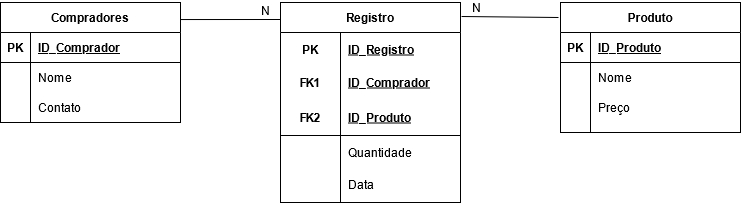
\includegraphics[width=\textwidth]{imgs/Diagram.png}

\newpage
\section*{Criação do Banco de Dados}

\begin{verbatim}
CREATE TABLE compradores (
    ID_comprador INT PRIMARY KEY NOT NULL AUTO_INCREMENT,
    nome_comprador VARCHAR(30) NOT NULL,
    contato VARCHAR(50)
);

CREATE TABLE produtos (
    ID_produto INT PRIMARY KEY NOT NULL AUTO_INCREMENT,
    nome_produto VARCHAR(30) NOT NULL,
    preco DECIMAL(5, 2) NOT NULL
);

CREATE TABLE registro_compras (
    ID_compra INT PRIMARY KEY AUTO_INCREMENT,
    qnt_compra TINYINT UNSIGNED NOT NULL,
    data_compra TIMESTAMP CURRENT_TIMESTAMP,
    ID_comprador INT,
    CONSTRAIN FK_ID_comprador FOREIGN KEY (ID_comprador)
        REFERENCES comprador(ID_comprador),
    ID_produto INT,
    CONSTRAIN FK_ID_produto FOREIGN KEY (ID_produto)
        REFERENCES produto(ID_produto)
);
\end{verbatim}

\newpage
\section*{Adicionando informações nas tabelas}

\begin{verbatim}
INSERT INTO compradores (nome_comprador, contato) VALUES ("Luiz", "@luiz123");
INSERT INTO compradores (nome_comprador, contato) VALUES ("Paulo", "@paul098");
INSERT INTO compradores (nome_comprador) VALUES ("Paulo");

INSERT INTO produtos (nome_produto, preco) VALUES ("Pão de Forma", 10.50);
INSERT INTO produtos (nome_produto, preco) VALUES ("Manteiga", 5.75);
INSERT INTO produtos (nome_produto, preco) VALUES ("Margarina", 6.00);
INSERT INTO produtos (nome_produto, preco) VALUES ("Requeijão", 8.50);
INSERT INTO produtos (nome_produto, preco) VALUES ("Biscoito", 7.50);
INSERT INTO produtos (nome_produto, preco) VALUES ("Leite", 10.00);
INSERT INTO produtos (nome_produto, preco) VALUES ("Toddy", 5.50);
INSERT INTO produtos (nome_produto, preco) VALUES ("Nescau", 13.00);

INSERT INTO registro_compras (qnt_compra, ID_comprador, ID_produto)
    VALUES (5, 1, 1);
INSERT INTO registro_compras (qnt_compra, ID_comprador, ID_produto)
    VALUES (3, 1, 3);
INSERT INTO registro_compras (qnt_compra, ID_comprador, ID_produto)
    VALUES (4, 1, 4);
INSERT INTO registro_compras (qnt_compra, ID_comprador, ID_produto)
    VALUES (2, 2, 6);
INSERT INTO registro_compras (qnt_compra, ID_comprador, ID_produto)
    VALUES (1, 2, 7);
\end{verbatim}

\newpage
\section*{Escolha dos tipos}

As escolhas foram bem padrões:
\begin{itemize}
    \item
        Os ids foram do tipo \texttt{INT}, são as chaves primárias.
    \item
        Os nomes foram do tipo \texttt{VARCHAR(30)}, nomes são strings.
    \item
        O contato segue a mesma lógica do nome, mas tem mais espaço.
    \item
        O preço foi do tipo \texttt{DECIMAL(5,2)} para que seja possível guardar números decimais (sem perda de precisão que o float tem).
    \item
        A qnt\_compra foi do tipo \texttt{TINYINT UNSIGNED}, não é possível comprar itens negativos e não é esperado mais de 255 itens.
    \item
        A data\_compra foi do tipo \texttt{TIMESTAMP}.
    \item
        A tabela registro\_compras possui duas chaves estrangeiras, são as referências para o comprador e produto.
\end{itemize}

\newpage
\section*{Exemplos de consultas}

\begin{itemize}
    \item Mostra o nome das pessoas que compraram mais que
        5 produtos iguais em uma única compra:
        \begin{verbatim}
    SELECT compradores.nome_comprador
    FROM compradores, registro_compra
    WHERE compradores.ID_comprador = registro_compra.ID_comprador
        AND registro_compra.qnt_compra >= 5
    GROUP BY compradores.nome_comprador
    ;
        \end{verbatim}
    \item Mostra o nome das pessoas que compraram "Biscoito",
        o timestamp em que foi comprado e
        quantos foram comprados:
        \begin{verbatim}
    SELECT compradores.nome_comprador,
        registro_compra.data,
        registro_compra.qnt_compra
    FROM compradores, registro_compra, produtos
    WHERE compradores.ID_comprador = registro_compra.ID_comprador
        AND produtos.ID_produto = registro_compra.ID_produto
        AND produtos.nome = "Biscoito"
    ;
        \end{verbatim}
    \item Mostra o nome das pessoas que gastaram mais de 10 reais em compras,
        o timestamp em que foi comprado,
        o nome e
        quantos desses produtos foram comprados:
        \begin{verbatim}
    SELECT compradores.nome_comprador,
        registro_compra.data,
        produtos.nome_produto,
        registro_compra.qnt_compra
    FROM compradores, registro_compra, produtos
    WHERE compradores.ID_comprador = registro_compra.ID_comprador
        AND produtos.ID_produto = registro_compra.ID_produto
        AND produtos.preco * registro_compra.qnt_compra >= 10
    ;
        \end{verbatim}
\end{itemize}

\end{document}
